\begin{pastexam}[label={px:ncku-109-ee-ds-05}]{成大電機所 109 學年度 第 5 題}
（問答；15 分）

Let $G=(V,E)$ be a weighted undirected graph with any two vertices connected by at most one edge
and $H$ be a subgraph of $G$ obtained by deleting an edge $e_i$ from $G$, i.e.,
$H=(V,E\text{-}\{e_i\})$. True or false? Explain if false. (15 points)
\begin{enumerate}[label=(\alph*)]
\item Minimal cost spanning tree of $G$ is unique.
\item The path from vertex $A$ to vertex $B$ on a minimal cost spanning tree of $G$ is a shortest
path from $A$ to $B$.
\item If the total cost of minimal cost spanning tree of $H$ is greater than that of $G$, then $e_i$
must be an edge in any minimal cost spanning tree of $G$.
\end{enumerate}
\end{pastexam}

\begin{pastsoln}
答案：(a) 錯，(b) 錯，(c) 對。 以下假設 $G$ 連通（才有生成樹）。

\textbf{(a) 錯}。 邊的權重有相同時，最小生成樹可能不只一棵。 反例：三角形 $A$、$B$、$C$，三條邊權重
都是 $1$。 任選兩條邊都是生成樹，成本都是 $2$，三棵都是最小生成樹。 只有在\textbf{所有邊權重都不同}
時，最小生成樹才保證唯一（資結書定理~24.4）。

\textbf{(b) 錯}。 最小生成樹讓\textbf{全部邊的總和}最小，不保證任兩點之間的路徑最短
（資結書第~24.5.4~節）。 反例：三角形，$w(A, B) = 2$、$w(B, C) = 2$、$w(A, C) = 3$。 最小生成樹是
$\{AB, BC\}$，成本 $4$（含 $AC$ 的兩棵成本都是 $5$）。 樹上 $A$ 到 $C$ 的路徑是 $A$--$B$--$C$，長度 $4$，
但直接走邊 $AC$ 只要 $3$。
\begin{center}
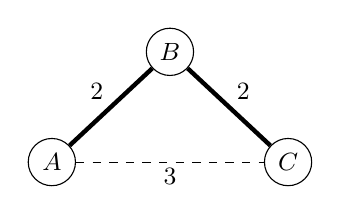
\begin{tikzpicture}[v/.style={circle,draw,minimum size=6mm,inner sep=0pt,font=\small},w/.style={font=\small,inner sep=2pt}]
\node[v] (A) at (0,0) {$A$};
\node[v] (B) at (1.5,1.4) {$B$};
\node[v] (C) at (3,0) {$C$};
\draw[line width=1.6pt] (A) -- node[w,above left] {2} (B);
\draw[line width=1.6pt] (B) -- node[w,above right] {2} (C);
\draw[dashed] (A) -- node[w,below] {3} (C);
\end{tikzpicture}
\end{center}

\textbf{(c) 對}。 \textbf{證明。} 用反證法。 假設 $G$ 有某一棵最小生成樹 $T$ 不含 $e_i$。 $T$ 的邊都在
$E - \{e_i\}$ 裡，而且連通 $V$ 的所有頂點，所以 $T$ 也是 $H$ 的生成樹。 於是 $H$ 的最小生成樹成本
$\le w(T)$，而 $w(T)$ 等於 $G$ 的最小生成樹成本，和「$H$ 的比 $G$ 的大」矛盾。 所以 $G$ 的每一棵最小
生成樹都含 $e_i$。 （若 $e_i$ 是橋，刪掉後 $H$ 不連通、沒有生成樹，把它的成本看成 $\infty$；這時 $G$ 的
每棵生成樹本來就都要用 $e_i$，結論同樣成立。）\hfill$\blacksquare$

反過來也對：若 $e_i$ 在 $G$ 的每一棵最小生成樹裡，刪掉它之後 $H$ 的最小生成樹成本一定比較大。
\end{pastsoln}
